\documentclass[12pt]{article}
\usepackage{graphicx}
\graphicspath{/}




\begin{document}
\Large{9.40 Intro to Neural Computation: pset1}
\section*{Problem 1: Random walk}
In P1 we consider a 500x1001 matrix X (randomwalk.mat) where each row represents the position of an object in microns as it takes a random walk for 1000 timesteps of 1ms.
\subsubsection*{Q1: Look at col1 of X to determine the positions of all patricles at t=0}

\scriptsize{Inspecting the first collumn of X we see that all particles starts at position 0.}

\subsubsection*{Q2: What is the value of t for the last collumn of X?}
Since there are 1001 cols and we begin counting at $t=0$ the 1000th col marks $t=1000ms=1s$
\subsubsection*{Q3:Plot the trajectory of particle 14 as a funtion of time}
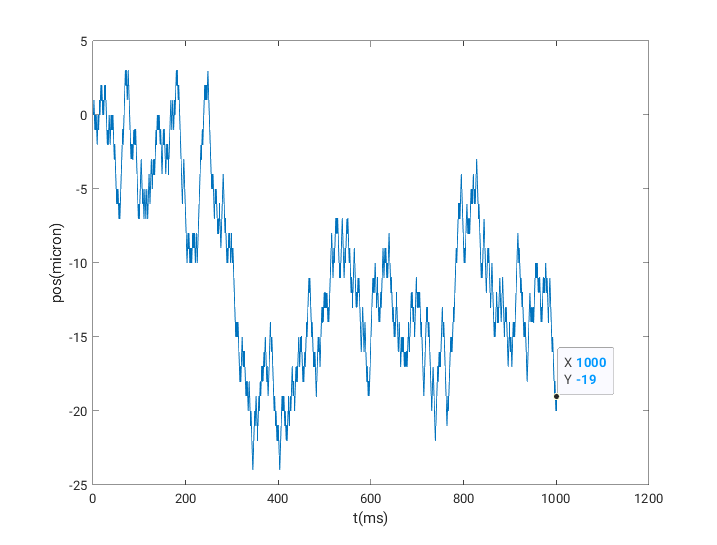
\includegraphics[width=0.9\textwidth]{rwof14.png}

\scriptsize{Like all the others it begins at $pos=0$, 14 ends up at $pos=-19$}  

\subsubsection*{Q4:In a single figure plot the trajectories of all the particles as a function of time. What do you see? Why each particle follows a different trajectory?}
\includegraphics*[width=0.9\textwidth]{alltrajecs.png}

We see that the trajectories when considered together resemble a normal distribution centerd at 0.\vspace{3mm}

At each time step each particle moves +1 or -1 with equal probability. So the probability of any patricular trajectory is 
$$ p = (\frac{1}{2})^{1000}$$
Let A be the event that at least two particles follow the same trajectory. Then the probability of A is given by: 
$$ P(A) = \sum_{i=2}^{500}{500 \choose i}*p^i$$
Which is an absurdly small number. To demonstrate this note that an upper bound for binomial coefficients is: ${k \choose i} \leq (\frac{ek}{i})^i$. So we can write: 
$$ P(A) \leq  \sum_{i=2}^{500}{(\frac{e500}{i2^{1000}})^i} \leq  499 \frac{e500}{2^{1001}} \approx 2\times10^{-296} $$  
So even a quite generous bound gives a probability which is as good as 0. 

\subsubsection*{Q5:Plot the mean displacement as a function of time is there any trend in this plot? Explain. }
\includegraphics*[width=0.9\textwidth]{avgdev.png}

The mean displacement seems to be growing logarithmically.

\end{document} 